\section{References}

\begin{frame}
  \frametitle{Books}
  \begin{columns}
    \column{0.85\textwidth}
    \small
    \begin{itemize}
    \item {\bf Mastering Embedded Linux, Second Edition, Packt
      Publishing}\\
      By Chris Simmonds, June 2017\\
      An up-to-date resource covering most aspects of embedded Linux
      development.\\
      \url{https://bit.ly/2A9Pb5Y}
    \item {\bf Embedded Linux Primer, Second Edition, Prentice Hall}\\
      By Christopher Hallinan, October 2010\\
      Covers a very wide range of interesting topics.\\
      \url{https://j.mp/17NYxBP}
    \item {\bf Embedded Linux System Design and Development}\\
      P. Raghavan, A. Lad, S. Neelakandan, Auerbach, Dec. 2005.
      Very good coverage of the POSIX programming API (still up
      to date).\\
      \url{https://j.mp/19X8iu2}
    \end{itemize}
    \normalsize
    \column{0.15\textwidth}
    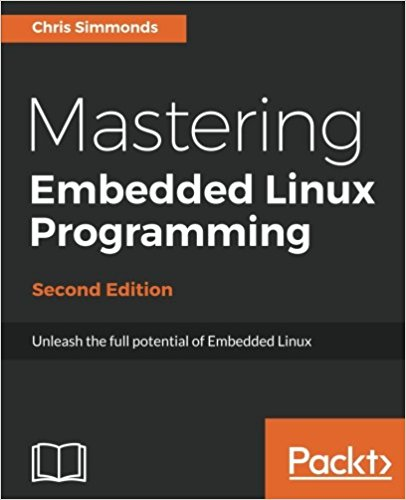
\includegraphics[height=0.25\textheight]{slides/sysdev-references/book-mastering-embedded-linux2.jpg}\\
    \vspace{0.5cm}
    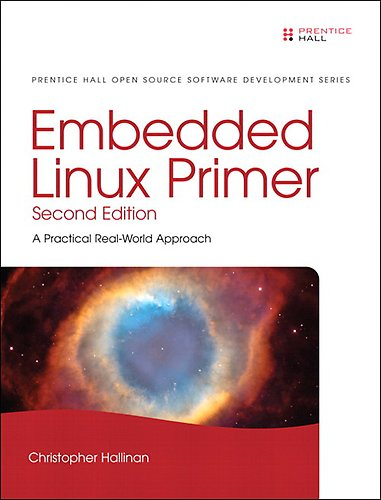
\includegraphics[height=0.25\textheight]{slides/sysdev-references/book-embedded-linux-primer2.jpg}\\
    \vspace{0.5cm}
    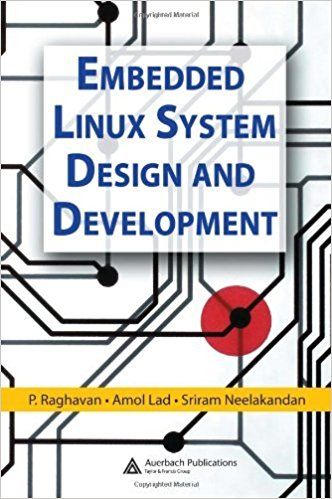
\includegraphics[height=0.25\textheight]{slides/sysdev-references/book-embedded-linux-sysdev.jpg}\\
  \end{columns}
\end{frame}

\begin{frame}
  \frametitle{Web sites}
  \begin{itemize}
  \item {\bf ELinux.org}, \url{https://elinux.org}, a Wiki entirely
    dedicated to embedded Linux. Lots of topics covered: real-time,
    filesystem, multimedia, tools, hardware platforms,
    etc. Interesting to explore to discover new things.
  \item {\bf LWN}, \url{https://lwn.net}, very interesting news site
    about Linux in general, and specifically about the kernel. Weekly
    edition, available for free after one week for non-paying
    visitors.
  \item {\bf Linux Gizmos}, \url{https://linuxgizmos.com}, a news site
    about embedded Linux, mainly oriented on hardware platforms
    related news.
  \end{itemize}
\end{frame}

\begin{frame}
  \frametitle{International conferences}
  Useful conferences featuring embedded Linux and kernel topics
  \begin{itemize}
  \item
    Embedded Linux Conference:
    
\includegraphics[width=0.35\textwidth]{slides/sysdev-references/elc-logo.png}\\
    \url{https://embeddedlinuxconference.com/}\\
    Organized by the Linux Foundation: USA (February-April), in Europe
    (October-November). Very interesting kernel and user space topics for embedded
    systems developers. Presentation slides and videos freely available
  \item Linux Plumbers, \url{https://linuxplumbersconf.org}\\
    Conference on the low-level plumbing of Linux: kernel, audio,
    power management, device management, multimedia, etc.
  \item FOSDEM: \url{https://fosdem.org} (Brussels, February)\\
    For developers. Presentations about system development.
  \end{itemize}
\end{frame}
